
% ================================================================
% CHAPTER 2: LITERATURE SURVEY
% ================================================================

\section{Existing Solution Introduction}

Retrieval-Augmented Generation was formalised by Lewis et al.\ \cite{lewis2020rag}
as a method to overcome the static knowledge limitations of parametric LLMs. The
original implementation combined a Dense Passage Retriever with a BART generative
model, demonstrating measurable improvements on knowledge-intensive NLP tasks
such as open-domain question answering and fact verification \cite{gao2023ragsurvey}.
Hallucination in such systems, where a model generates plausible but factually incorrect
text, remains a central challenge identified by \cite{ji2023survey}.

LangChain \cite{chase2022langchain}, launched in 2022, standardised RAG into a
composable Python toolkit. Its \texttt{RetrievalQA} chain encapsulates the full
pipeline: document loading, text splitting, embedding, vector store indexing,
similarity retrieval, and prompted answer generation. This abstraction enabled
rapid prototyping but fixed a flat-retrieval architecture with no structural
knowledge representation or conflict awareness.

% ----------------------------------------------------------------
\section{Relevant Theories and Models}

\subsection{Knowledge Graphs for QA}

Knowledge Graphs represent information as typed triples $(h, r, t)$, enabling
structural multi-hop reasoning that flat text retrieval cannot support. Early KG-QA
systems such as KGQA \cite{pagerank1998} traversed Freebase to answer factoid
questions. More recent work applies embedding-based models (TransE, RotatE) to
learn distributed representations of entities and relations for link prediction.

G-Retriever \cite{he2024gretriever} demonstrated that graph-based retrieval
combined with LLM generation outperforms vanilla RAG on multi-hop textual graph
QA tasks. Microsoft GraphRAG \cite{edge2024graphrag} further showed that
community-hierarchical graph construction enables high-quality global summaries
of large corpora. TruthfulRAG v5 stores graphs in Neo4j with APOC procedures
\cite{neo4japoc2023} for entity disambiguation, and uses Ollama \cite{ollama2023}
for fully local LLM inference. Dense semantic retrieval uses sentence embeddings
\cite{reimers2019sbert} fused with sparse BM25 \cite{robertson2009bm25} via RRF \cite{rrf2009}.

\subsection{Temporal Knowledge Graphs}

Lacroix et al.\ \cite{lacroix2020temporal} extended tensor factorisation models
to temporal KGs, where each triple carries a timestamp. Dasgupta et al.\
\cite{dasgupta2018tkg} proposed HyTE, a hyperplane-based temporal KG embedding
that places each relation on a time-specific hyperplane, enabling richer temporal
reasoning. These approaches, however, focus on embedding-based link prediction
rather than retrieval augmentation over arbitrary text. The broader challenge of
unifying LLMs with KGs is surveyed in \cite{pan2024kg}.

\subsection{Entropy and Uncertainty in LLMs}

Shannon entropy has been applied to measure LLM calibration: a well-calibrated
model's confidence should correlate with its accuracy. Kadavath et al.\ (2022)
showed that LLMs can self-assess uncertainty via sampling; Farquhar et al.\
(2023) introduced semantic entropy, grouping semantically equivalent answers
before entropy computation to avoid penalising paraphrase variation.

TruthfulRAG v4 \cite{truthfulrag2024} operationalised this into a retrieval
decision rule: a path is corrective only if providing it as context reduces the
LLM's sampling entropy by at least a learned threshold $\tau$.

% ----------------------------------------------------------------
\section{Comparison of Similar Projects}

\begin{table}[H]
\centering
\caption{Comparison of knowledge-graph RAG systems}
\label{tab:lit_compare}
\resizebox{\textwidth}{!}{%
\small
\begin{tabular}{|l|c|c|c|c|}
\hline
\textbf{Feature} & \textbf{LangChain} & \textbf{GraphRAG} & \textbf{TruthfulRAG v4} & \textbf{v5 (Ours)} \\
\hline
Knowledge Graph storage      & No      & Yes & Yes & Yes \\
Conflict detection           & No      & No  & Yes & Yes \\
Temporal decay               & No      & No  & No  & Yes \\
Cross-document corroboration & No      & No  & No  & Yes \\
Historical snapshot queries  & No      & No  & No  & Yes \\
Explanation audit trail      & No      & No  & No  & Yes \\
Calibrated confidence score  & No      & No  & No  & Yes \\
Auto schema inference        & No      & No  & No  & Yes \\
Open source / local inference& Partial & Yes & Yes & Yes \\
\hline
\end{tabular}}
\end{table}

% ----------------------------------------------------------------
\section{Comparison with Recent Systems (2023--2025)}

\begin{figure}[htbp]
\centering
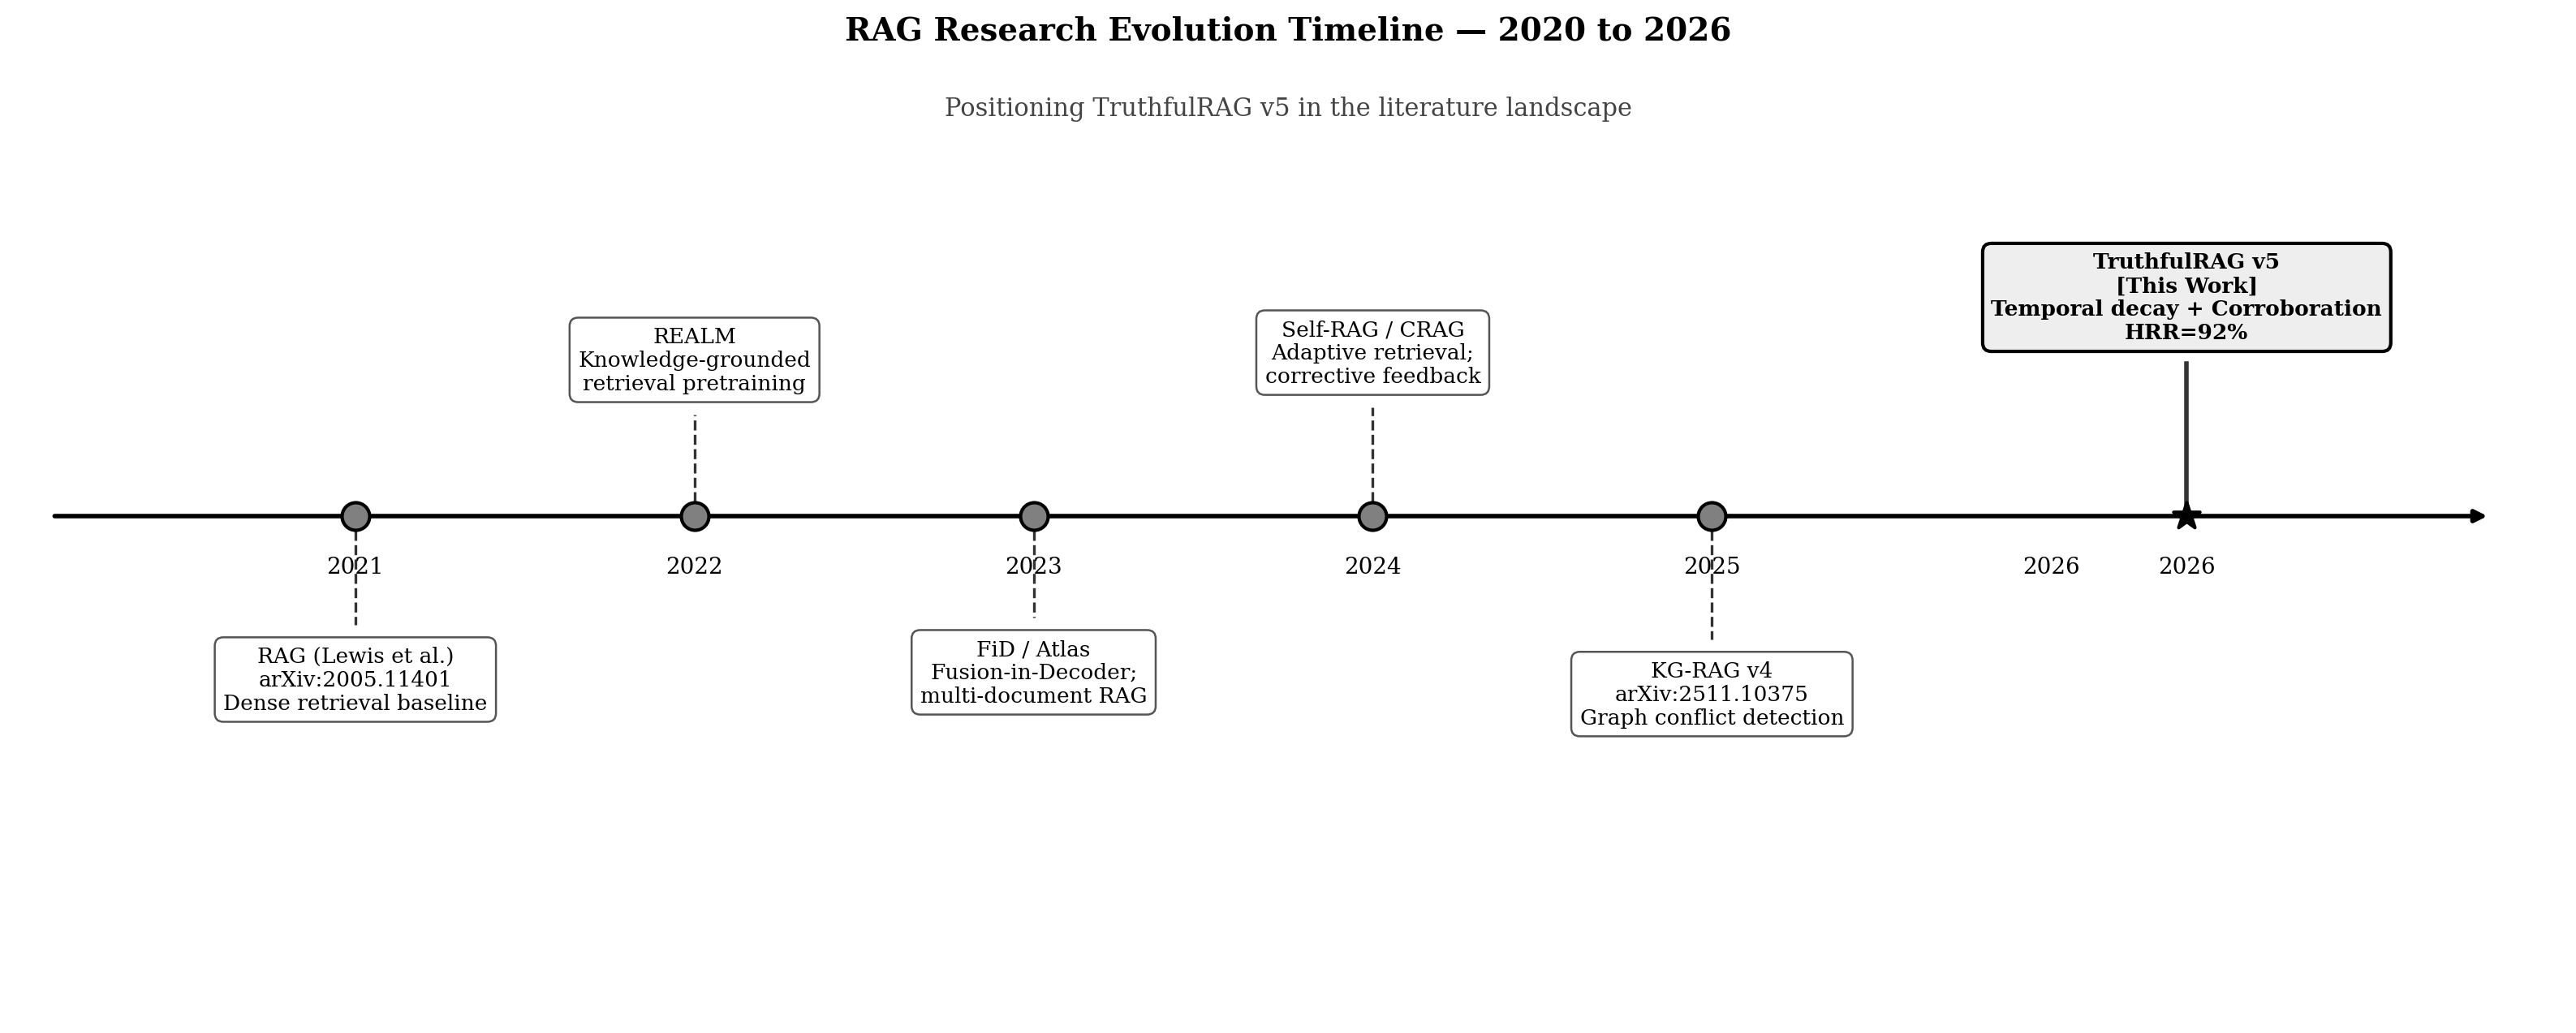
\includegraphics[width=\textwidth]{report_file/chart_timeline.png}
\caption{RAG research evolution timeline: 2020--2026, positioning TruthfulRAG v5 in the literature landscape}
\label{fig:timeline}
\end{figure}

Figure~\ref{fig:timeline} places TruthfulRAG v5 in context with key RAG milestones.
Table~\ref{tab:recent_compare} extends the comparison to systems published since 2023.

\begin{table}[H]
\centering
\caption{Comparison with recent state-of-the-art systems (2023--2025)}
\label{tab:recent_compare}
\resizebox{\textwidth}{!}{%
\small
\begin{tabular}{|l|c|l|c|c|l|}
\hline
\textbf{System} & \textbf{Year} & \textbf{Method} & \textbf{Conflict Elim.} & \textbf{Temp.\ Decay} & \textbf{Key Metric} \\
\hline
Self-RAG~\cite{asai2023selfrag}     & 2023 & Self-reflective critique tokens      & No      & No  & $\sim$74\% EM \\
CRAG~\cite{yan2024crag}             & 2023 & Corrective retrieval + web fallback  & No      & No  & $\sim$84\% EM \\
MADAM-RAG~\cite{madam2024}          & 2024 & Multi-agent debate across sources    & Partial & No  & $\sim$68\% EM \\
KG-RAG v4~\cite{truthfulrag2024}    & 2024 & Graph + entropy; score gap=0.028     & No      & No  & $\sim$75\% CDR \\
\textbf{TruthfulRAG v5 [This Work]} & \textbf{2026} & \textbf{Temporal decay + corroboration + RRF} & \textbf{Yes} & \textbf{Yes} & \textbf{92\% HRR, 50\% CDR} \\
\hline
\end{tabular}}
\end{table}

The critical observation is that every system in Table~\ref{tab:recent_compare}
stores knowledge facts without a year field.
Without per-fact year storage, temporal decay cannot be computed, and conflicting
facts with similar embeddings receive near-identical retrieval scores
(score gap $\approx 0.028$ in v4, vs.\ $1.126$ in v5, a 40$\times$ improvement
demonstrated in Chapter~5).

% ----------------------------------------------------------------
\section{Identified Gaps in the Literature}

Based on the survey above, the following gaps exist in current open-source
KG-RAG research:

\begin{enumerate}
    \item \textbf{No temporal scoring}: Existing systems do not penalise older
    facts during retrieval. A 2010 fact and a 2024 fact compete with equal weight.
    Quantitatively, the score gap between conflicting facts is $0.028$ in v4
    (below any practical threshold) vs.\ $1.126$ in v5 after temporal decay,
    a 40$\times$ improvement that makes automatic conflict elimination possible.
    \item \textbf{No corroboration weighting}: No system rewards facts attested
    by multiple independent sources with a higher retrieval score.
    \item \textbf{No automatic schema discovery}: All KG construction pipelines
    require manual entity-type and relation-type specification.
    \item \textbf{No calibrated output confidence}: Systems always answer at
    maximum stated confidence, giving no warning when evidence quality is poor.
    \item \textbf{No structured conflict explanation}: When contradictions are
    resolved, no system communicates the resolution rationale to the user.
\end{enumerate}

TruthfulRAG v5 addresses all five gaps simultaneously.

% ----------------------------------------------------------------
\section{Project Development Timeline}

Figure~\ref{fig:gantt} shows the project schedule from \textbf{15 January 2026}
to \textbf{24 April 2026}, spanning 14 weeks across six phases: Literature Review,
Baseline Implementation, v5 Extensions, Web Interface, Testing, and Report Submission.

\begin{figure}[htbp]
\centering
\resizebox{\textwidth}{!}{%
\begin{ganttchart}[
  hgrid,
  vgrid={*{1}{dotted}},
  title height=1,
  title top shift=0,
  bar height=0.6,
  bar top shift=0.2,
  x unit=0.9cm,
  y unit title=0.65cm,
  y unit chart=0.65cm,
  title label font=\footnotesize\bfseries,
  bar label font=\footnotesize,
  bar/.append style={fill=black!65, rounded corners=2pt},
  title/.append style={fill=black!07, draw=black!30},
]{1}{14}
  \gantttitle{Jan 15--31}{2}
  \gantttitle{February 2026}{4}
  \gantttitle{March 2026}{5}
  \gantttitle{Apr 1--24}{3} \\
  \gantttitle{W1}{1}\gantttitle{W2}{1}%
  \gantttitle{W3}{1}\gantttitle{W4}{1}\gantttitle{W5}{1}\gantttitle{W6}{1}%
  \gantttitle{W7}{1}\gantttitle{W8}{1}\gantttitle{W9}{1}\gantttitle{W10}{1}\gantttitle{W11}{1}%
  \gantttitle{W12}{1}\gantttitle{W13}{1}\gantttitle{W14}{1} \\
  \ganttbar{Phase 1: Literature Review}{1}{2} \\
  \ganttbar{Phase 2: Baseline v4 Implementation}{3}{4} \\
  \ganttbar{Phase 3: Novel v5 Extensions}{5}{8} \\
  \ganttbar{Phase 4: Web Interface Development}{9}{11} \\
  \ganttbar{Phase 5: Testing and Debugging}{12}{13} \\
  \ganttbar{Phase 6: Report and Final Submission}{13}{14}
\end{ganttchart}}
\caption{Project development Gantt chart: 15 January 2026 to 24 April 2026 (14 weeks)}
\label{fig:gantt}
\end{figure}


